\subsection{M1U: Ungesteuerter Einpuls-Gleichrichter}

% --- bestehende Grafik: Schaltung ---
\begin{center}
    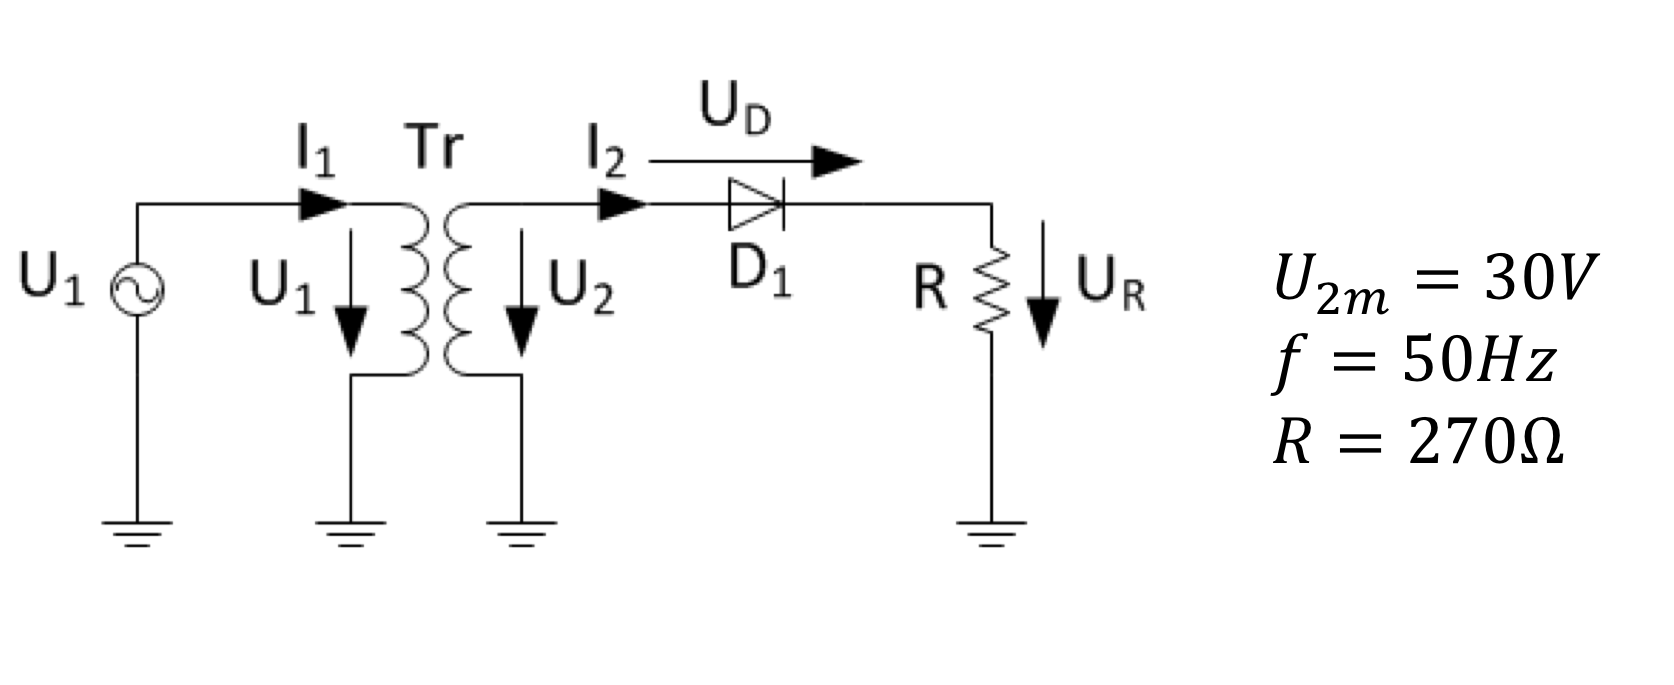
\includegraphics[width=0.85\linewidth]{images/M1U.png}
\end{center}

Der ungesteuerte Einpuls-Gleichrichter besteht aus einer Diode und einer einphasigen Wechselspannungsquelle.
Er arbeitet ohne Stellmöglichkeit und liefert eine pulsierende Gleichspannung mit der Pulszahl $p=1$.

Eingangsspannung:
\[
u_s(t) = \hat U \sin(\omega t)
\]
mit:
\begin{itemize}
\item $\hat U$: Scheitelwert der Eingangsspannung,
\item $\omega = 2\pi f$: Kreisfrequenz,
\item $f$: Netzfrequenz.
\end{itemize}

Momentane Ausgangsspannung:
\[
u_d(t) =
\begin{cases}
\hat U \sin(\omega t), & \sin(\omega t) \ge 0, \\
0, & \sin(\omega t) < 0.
\end{cases}
\]

Mittelwert der Gleichspannung:
\[
\cbl{\overline{u_d} = \frac{1}{2\pi}\int_0^{\pi} \hat U \sin\gamma \, d\gamma
= \frac{\hat U}{\pi}}
\]
mit:
\begin{itemize}
\item $\gamma = \omega t$: elektrischer Winkel.
\end{itemize}

Effektivwert der Ausgangsspannung:
\[
\cbl{U_{d,\mathrm{RMS}} = \sqrt{\frac{1}{2\pi}\int_0^{\pi} \hat U^2 \sin^2\gamma \, d\gamma}
= \frac{\hat U}{2}}
\]

Mittelwert des Gleichstroms bei ohmscher Last $R$:
\[
\cbl{I_d = \frac{\overline{u_d}}{R} = \frac{\hat U}{\pi R}}
\]

Effektivwert des Stroms:
\[
\cbl{I_{d,\mathrm{RMS}} = \frac{U_{d,\mathrm{RMS}}}{R} = \frac{\hat U}{2R}}
\]

Leistungsaufnahme an ohmscher Last:
\[
\cbl{P = R I_{d,\mathrm{RMS}}^2 = \frac{\hat U^2}{4R}}
\]

Eigenschaften:
\begin{itemize}
\item Keine Stellmöglichkeit der Ausgangsspannung.
\item Sehr hohe Restwelligkeit der Gleichspannung.
\item Geringe Gleichspannungsqualität.
\item Einfachste Gleichrichterschaltung.
\end{itemize}

% --- bestehende Grafik: Spannungsverlauf ---
\begin{center}
    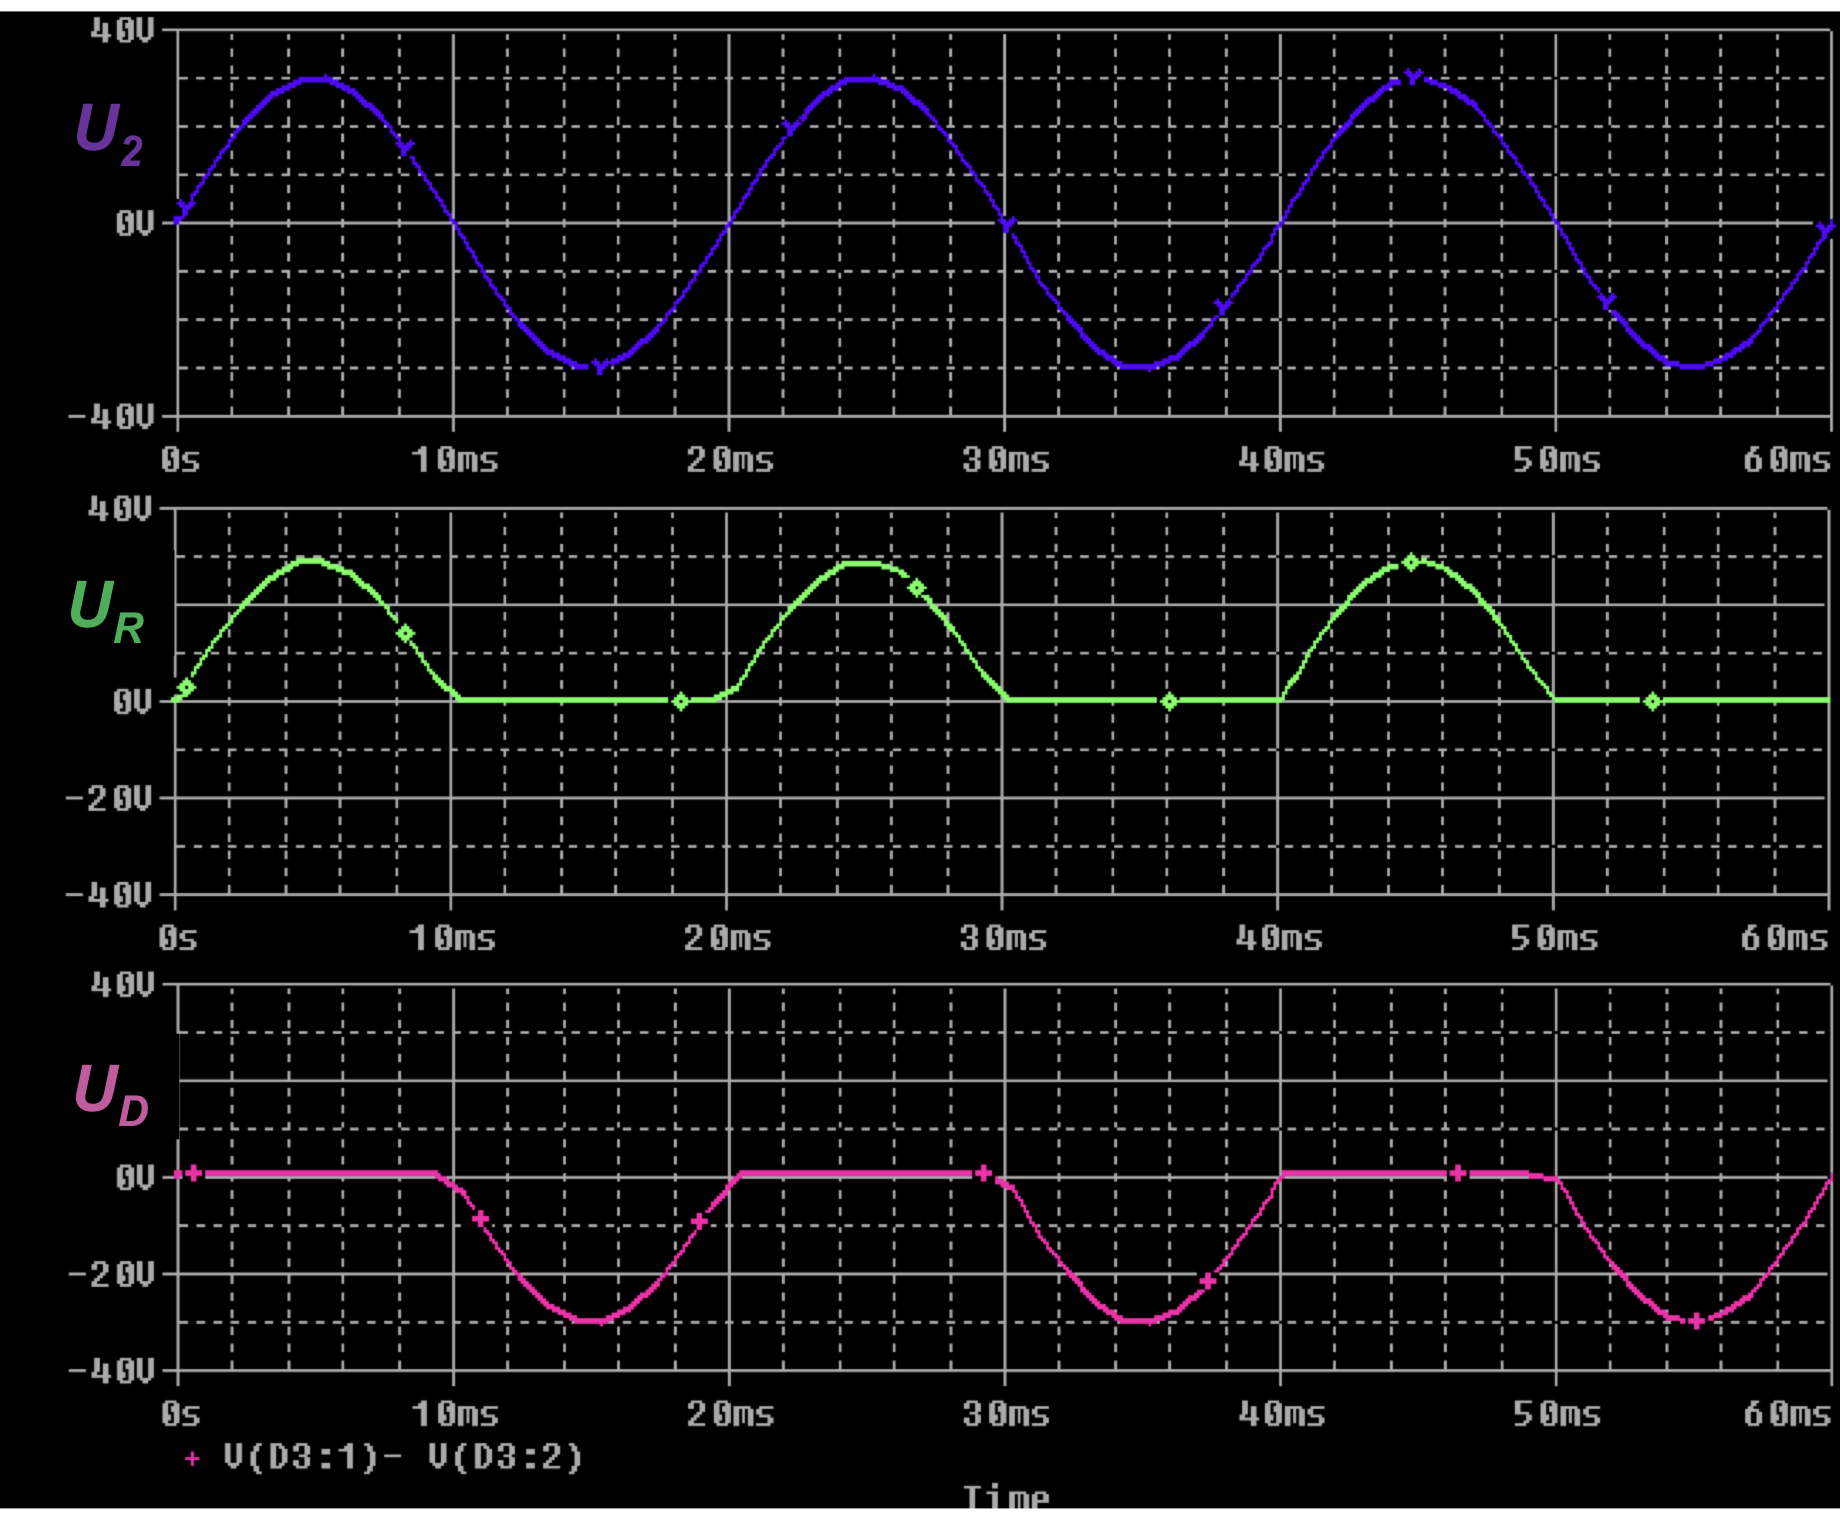
\includegraphics[width=0.85\linewidth]{images/M1U_verlauf.png}
\end{center}

\subsection{M1C: Gesteuerter Einpuls-Gleichrichter}

% --- bestehende Grafik: Schaltung ---
\begin{center}
    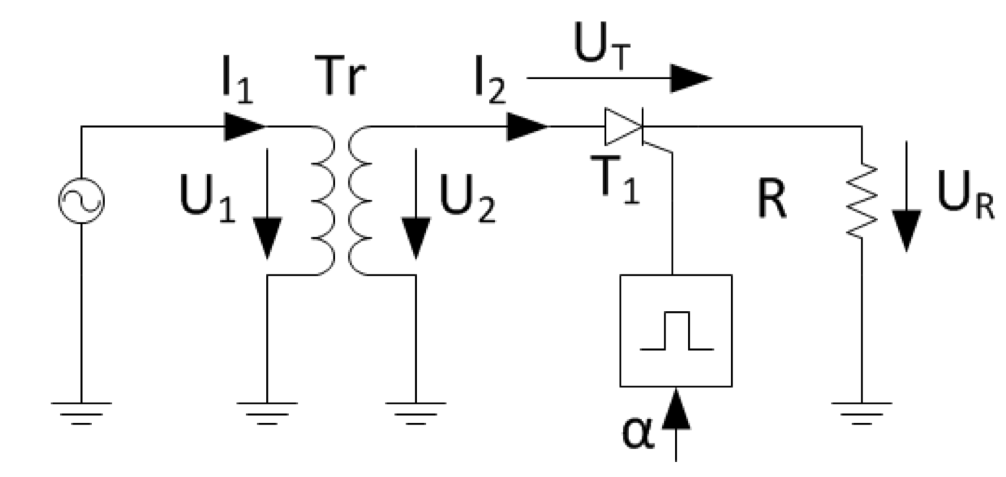
\includegraphics[width=0.85\linewidth]{images/M1C.png}
\end{center}

Der gesteuerte Einpuls-Gleichrichter ersetzt die Diode durch einen Thyristor.
Der Leitbeginn wird durch den Zündwinkel $\alpha$ gesteuert.

Eingangsspannung:
\[
u_s(t) = \hat U \sin(\omega t)
\]
mit:
\begin{itemize}
\item $\hat U$: Scheitelwert der Eingangsspannung,
\item $\omega = 2\pi f$: Kreisfrequenz,
\item $f$: Netzfrequenz.
\end{itemize}

Leitbedingung:
\[
\boxed{\omega t \ge \alpha}
\]

Momentane Ausgangsspannung:
\[
u_d(t) =
\begin{cases}
\hat U \sin(\omega t), & \omega t \ge \alpha, \\
0, & \omega t < \alpha.
\end{cases}
\]

Mittelwert der Gleichspannung:
\[
\cbl{\overline{u_d}
= \frac{1}{2\pi}\int_{\alpha}^{\pi} \hat U \sin\gamma \, d\gamma
= \frac{\hat U}{2\pi}(1+\cos\alpha)}
\]

Stellbereich:
\[
0 \le \alpha \le \pi
\]

Grenzfälle:
\[
\alpha = 0 \Rightarrow \overline{u_d} = \frac{\hat U}{\pi}
\]
\[
\alpha = \pi \Rightarrow \overline{u_d} = 0
\]

Mittelwert des Stroms bei ohmscher Last $R$:
\[
\cbl{I_d = \frac{\overline{u_d}}{R}
= \frac{\hat U}{2\pi R}(1+\cos\alpha)}
\]

Effektivwert der Ausgangsspannung:
\[
\cbl{U_{d,\mathrm{RMS}}
= \sqrt{\frac{1}{2\pi}\int_{\alpha}^{\pi} \hat U^2 \sin^2\gamma \, d\gamma}}
\]

Leistungsaufnahme an ohmscher Last:
\[
\cbl{P = R I_{d,\mathrm{RMS}}^2}
\]

Eigenschaften:
\begin{itemize}
\item Stellbare Gleichspannung über den Zündwinkel $\alpha$.
\item Bei $\alpha = 0$: Verhalten wie M1U.
\item Bei $\alpha > 90^\circ$: negativer Mittelwert möglich (in geeigneter Schaltung Rückspeisung).
\item Einfachster gesteuerter Gleichrichter.
\end{itemize}

% --- bestehende Grafik: Spannungsverlauf ---
\begin{center}
    \includegraphics[width=0.85\linewidth]{images/M1C_verlauf.png}
\end{center}
